\section{Modularisierung}

Ziel der Modularisierung ist eine \textbf{Reduktion der Komplexität.}
$$ \sum_{i} \text{complexity(problem)}_i < \text{complexity} \Big( \sum_{i} \text{problem}_i \Big) $$

\vspace{-0.2cm}


\subsection{Grundprinzip Modularisierung}

\begin{outline}
    \1 \textbf{Problem in (einfachere) Unterprobleme aufteilen} und diese Unterprobleme jeweils \textbf{einzeln angehen}
    \1 Abstraktion 
\end{outline}


\subsubsection{Motivation für Modularisierung}

\begin{outline}
    \1 \textbf{Grosse Projekte -- 'richtige' Softwaresysteme}
        \2 Systematischer Designansatz und strukturierter Aufbau ermöglichen effiziente \textbf{Arbeit im Team}
        \2 Schnittstellen müssen klar definiert werden
    \1 \textbf{Informatin Hiding}
        \2 Für die Nutzung eines Moduls (Unit) muss es gnügen, \textbf{nur die Schnittstellen} zu kennen
\end{outline}


\subsubsection{Phasenunterteilung beim Entwurf}

\begin{outline}
    \1 \textbf{Grobentwurf, Architektur (architectural design)}
        \2 (Software-) System im Grossen
        \2 Schnittstellen zu anderen (Nicht-Software-) Systemen
        \2 Datenstruktur im Grossen
        \2 \textbf{Aufteilung in Subsysteme}
        \2 \textbf{Schnittstellen zwischen Subsystemen}
    \1 \textbf{Feinentwurf}
        \2 Innenleben und Datenstruktur im Kleinen
\end{outline}


\subsection{Bewertung einer Zerlegung}

\begin{outline}
    \1 \textbf{Kopplung (coupling)}
        \2 Mass für Komplexität der Schnittstelle
    \1 \textbf{Kohäsion (cohesion)}
        \2 Aussage, wie stark eine funktionale Einheit wirklich zusammengehört
        \2 Mass die die Stärke des inneren Zusammenhangs
\end{outline}

\vspace{0.1cm}

\textbf{ \textrightarrow\ Ziel ist eine schwache Kopplung mit starker Köhäsion!}


\subsection{Kopplung}

\vspace{-0.2cm}

\begin{tikzpicture}[baseline=(current bounding box.north), >=latex]
    \node[anchor=north west] (kopplung) {
        \begin{minipage}{0.8\columnwidth}
            \begin{outline}
                \1 \textbf{Keine direkte Kopplung}
                \1 \textbf{Datenkopplung}
                    \2 Kommunikation ausschliesslich über Parameter
                \1 \textbf{Datenbereichskopplung}
                    \2 Ein Modul hat Zugriff auf eine Datenstruktur eines anderen Moduls. Es werden allerdings nur einzelne
                        Komponenten wirklich benötigt.
                \1 \textbf{Steuerflusskopplung} (control flow)
                    \2 Ein Modul beeinflusst Steuerfluss eines anderen Moduls
                \1 \textbf{Globale Kopplung}
                    \2 Kommunikation über globale Variablen, jedes Modul hat Zugriff
                \1 \textbf{Inhaltskopplung (Todsünde!)}
                    \2 Aus einem Modul heraus werden lokale Daten eines anderen Moduls modifiziert, obwohl dieses Modul
                        gar nicht vom anderen Modul aufgerufen wird.
            \end{outline}
        \end{minipage}
    };

    % Vertical arrow
    \draw[->, thick] ([xshift=-1em]kopplung.south west) -- ([xshift=-1em]kopplung.north west)
        node[very near start, left, color=red, thick]   {\shortstack{ \textbf{stark} \\ \textbf{(schlecht)}} }
        node[very near end, left, color=green]          {\shortstack{ \textbf{schwach} \\ \textbf{(gut)}} };
\end{tikzpicture}


\subsection{Kohäsion}

\vspace{-0.2cm}

\begin{tikzpicture}[baseline=(current bounding box.north), >=latex]
    \node[anchor=north west] (cohesion) {
        \begin{minipage}{0.8\columnwidth}
            \begin{outline}
                \1 \textbf{funktional}
                    \2 Die Teile einer Einheit bilden zusammen eine Funktion, bzw. eine Funktionsgruppe
                \1 \textbf{sequentiell}
                    \2 Teilfunktionen einer Einheit werden nacheinander ausgeführt, wobei das Resultat einer
                        Funktion als Eingabe für die nächste verwendet wird
                \1 \textbf{kommunikativ}
                    \2 Die Teilfunktionen einer Einheit werden auf den gleichen Daten ausgeführt, Reihenfolge
                        spielt keine Rolle
                \1 \textbf{prozedural}
                    \2 Teilfunktionen werden nacheinander ausgeführt, verknüpft über Steuerfluss
                \1 \textbf{\cbl{zeitlich}}
                    \2 Die Teile einer Einheit sind alle zu einer bestimmten Zeit auszuführen
                    \2 Typischer Fall: alle Initialisierungsfunktionen werden zusammengefasst
                \1 \textbf{logisch}
                    \2 (nicht zusammengehörende) Teilfunktionen einer Einheit gehören zu einer Einheit
                \1 \textbf{zufällig}
                    \2 Die Teilfunktionen einer Einheit haben keinen sinnvollen Zusammenhang
            \end{outline}
        \end{minipage}
    };

    % Vertical arrow
    \draw[->, thick] ([xshift=-1em]cohesion.south west) -- ([xshift=-1em]cohesion.north west)
        node[very near start, left, color=red, thick]   {\shortstack{ \textbf{schwach} \\ \textbf{(schlecht)}} }
        node[very near end, left, color=green]          {\shortstack{ \textbf{stark} \\ \textbf{(gut)}} };
\end{tikzpicture}


\subsubsection{Ziele bezüglich Kohäsion}

\begin{outline}
    \1 Kohäsion soll maximiert werden \\
        \textbf{ \textrightarrow\ starke Kohäsion führt automatisch zu schwacher Kopplung!}
    \1 Den genauen Wert der Kohäsion zu ermitteln ist \textbf{kein} Ziel
\end{outline}

\vspace{0.1cm}

\textbf{ \textrightarrow\ Zusammengehörendes zusammennehmen!}


\subsection{Guidelines -- gute Modularisierung}

\begin{outline}
    \1 \textbf{Zusammengehörendes zusammennehmen}
        \2 Defines für spezigisches Modul in Header-File des Moduls
    \1 Passende / aussagekräftige Namen für Variablen
    \1 'Interne' (private) Funktionen in \mylstbox{.c}-file deklarieren und definieren
    \1 Schnittstellenbeschreibung in Header-Dateien
        \2 Falls möglich: Doxygen verwenden
    \1 Lokale Funktionen (z.B. in \mylstbox{main.c}) bei Funktionsdeklarationen kommentieren
    \1 Allenfalls 'globalen' Header für Typdefinitionen
        \2 besser: Typen aus \mylstbox{stdint.h} verwenden
    \1 \mylstbox{uint8_t} etc. verwenden, wenn gezielt ein 8 Bit register angesprochen wird (und nur dann!)
    \1 Keine \mylstbox{initialization.h} Dateien \textrightarrow\ zeitliche Kohäsion!
        \2 generell keine Dateien wie: \mylstbox{global.h}, \mylstbox{defines.h}, \mylstbox{util.h}, \mylstbox{project.h}
\end{outline}

\vspace{0.2cm}

\textbf{Hinweis:} Für die Zurechtfindung in einem bestehenden Projekt müssen generell immer zuerst die \textbf{Header-Files studiert werden!}


\example{Schlechte vs. gute Modularisierung}

\begin{minipage}[t]{0.48\columnwidth}
    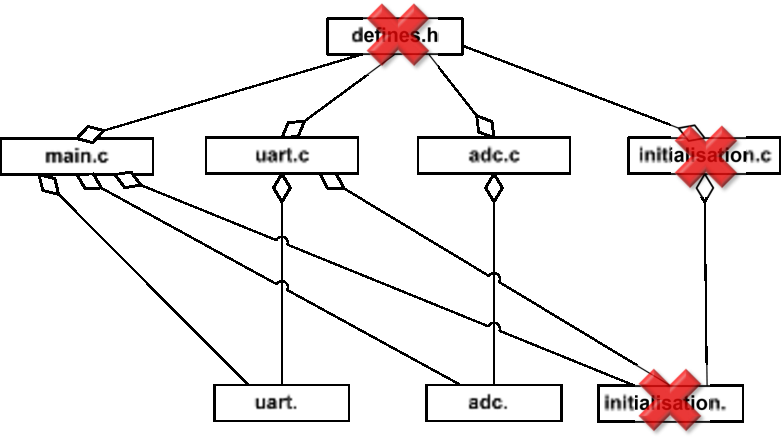
\includegraphics[width=\columnwidth, align=t]{images/modulaisierung_bsp_schlecht.pdf}
\end{minipage}
\hfill
\begin{minipage}[t]{0.48\columnwidth}
    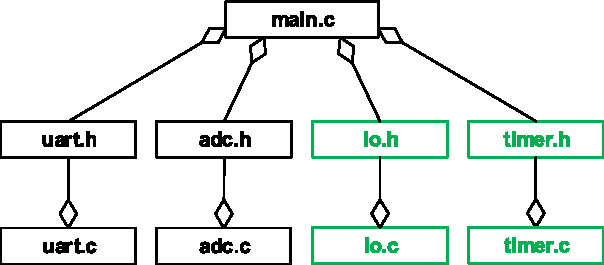
\includegraphics[width=\columnwidth, align=t]{images/modulaisierung_bsp_gut.pdf}
\end{minipage}


\subsection{Package-Diagramm}

\begin{outline}
    \1 Ein Package besteht aus mindestens einer, üblich aus mehreren Klassen, die zusammengehören (Stichwort: \textbf{Kohäsion})
    \1 Im Package-Diagramm kann dargestellt werden, welche Packages mit welchen anderen Packages Verbindungen haben (dürfen) 
        \2 \textbf{Abhängigkeiten zwischen Packages} können sichtbar gemacht werden
    \1 Packagekonzept in C++: Namespaces umgesetzt
        \2 ein Namespace entspricht einem Package
\end{outline}


\example{Schlechtes vs. gutes Packaging}

\begin{center}
    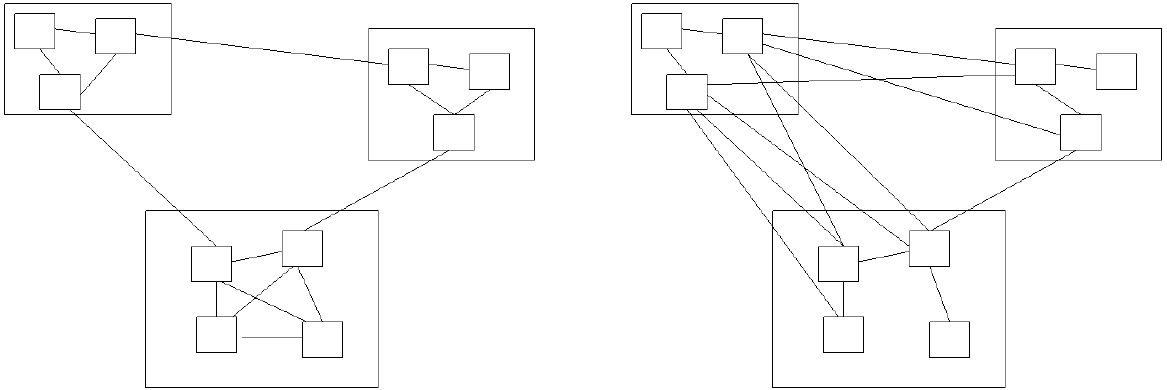
\includegraphics[width=0.9\columnwidth]{images/modulaisierung_bsp.png}
\end{center}

links: hohe Kohäsion, tiefe Kopplung \textrightarrow\ gut \\
rechts: tiefe Kohäsion, hohe Kopplung \textrightarrow\ schlecht

